\documentclass[11pt,letterpaper]{article}
\usepackage[spanish]{babel}
\usepackage{graphicx}
\usepackage[right=2cm,left=3cm,top=2cm,bottom=2cm,headsep=0cm,footskip=0.5cm]{geometry}


\title{INFORME DE INTERRUPCIONES}
\author{Liliana Marcela Barbosa Esteban\\% <-this % stops a space
Universidad de Antioquia \\
Curso: Informática II
}
\date{}

%%%%%%%%%%%%%%%%%%%%%%%%%%%%%%%%%%%%%%%%%%%%%%%%%%%%%%%%%%%%%%%%%%%%%%%%%%%%%%%%

\begin{document}


\maketitle
\thispagestyle{empty}
\pagestyle{empty}

\section{INTRODUCCIÓN}
El ser humano desde la antigüedad ha buscado la manera de crear artefactos que procesen información o datos de una manera automática, es por ello que ha inventado maquinas como la Antikythera, la calculadora de Pascal, la máquina analítica de Charles Babbage, hasta llegar al primer computador en los años 40. Adicionalmente, después de la segunda guerra mundial fue creado el transistor y el circuito integrado lo cual permitió el paso a el desarrollo de los microprocesadores en los años 70 y el desarrollo tecnológico de hoy en día.
\newline
\newline
Es importante mencionar que el microprocesador es el resultado de la miniaturización de la electrónica digital implementándose en el circuito integrado y posteriormente aumentando su rapidez y rendimiento. Además, en todo dispositivo electrónico está presente el microprocesador y actúa como la unidad central de procesamiento de la máquina. Precisamente ese dispositivo es el encargado de dar instrucciones asociadas al tratamiento de la información. Cabe resaltar que para llevar a cabo aquel proceso, se hace una ejecución secuencial de instrucciones a menos que se ejecute alguna función que altere aquel orden.
\newline
\newline
Aquel tipo de funciones que alteran el orden de instrucciones principales, se efectúan gracias a las interrupciones en el microprocesador. Es decir, mediante el mecanismo que permite llevar a cabo un evento asíncrono que cumple con una serie de condiciones para que se ejecute en un determinado instante.
\newline
\newline
Teniendo en cuenta que en estos últimos años los microprocesadores forman parte de la mayoría de los elementos con los que se interactúa día a día, es de gran importancia aprender cómo es el funcionamiento de estos elementos denominados por muchos como el “cerebro” de las máquinas. Por consiguiente, es necesario comenzar con las interrupciones ya que es un mecanismo muy potente que está presente en ellos, y permiten la suspensión de la secuencia del curso y realizar ciertas acciones de mayor prioridad. 
\newline
\newline
Para este trabajo se toma de referencia un conjunto de documentos y páginas web con información verídica, donde los autores explican desde diferentes puntos las interrupciones a nivel de los microprocesadores y realizan ejemplos respecto a ese asunto. Por otra parte, cabe resaltar que el tema se aborda de manera expositiva, retomando una parte de la historia de ese mecanismo y concluyendo en la importancia de éste.
\newline

%%%%%%%%%%%%%%%%%%%%%%%%%%%%%%%%%...................................%%%%%%%%%%%%%%%%%%%%%%%%%%%%%%%%%

\section{CUERPO DEL TRABAJO}
Existen situaciones de las cuales sólo se conoce que están asociadas a un proceso y que ha ocurrido. Para ello se elige una serie de condiciones que muestra en qué instante debe ser atendido el evento. Básicamente, el papel de determinar en qué momento debe ejecutarse cierta acción hace parte de las interrupciones.
\newline
\newline
No obstante, las interrupciones a nivel del microprocesador no están muy alejadas de lo que sería de manera general. De hecho, son un mecanismo potente que mejora eficazmente algún programa que deba procesar el circuito integrado y se hace mediante el salto a una subrutina. La decisión de pasar a otra serie de instrucciones la toma el procesador al evaluar si la solicitud que llega (mediante un mecanismo de \textit{hardware}) es de mayor prioridad que la secuencia en curso.
\newline
\newline
Por otra parte, es importante mencionar que las interrupciones nacen de la carencia de métodos que permitieran llevar información periférica al procesador principal de un conjunto de elementos electrónicos que interactúan entre sí. Además, el tipo de evaluación de las interrupciones no fue siempre de la misma manera, de hecho, antes no se trataba a través de la unidad de interrupciones sino con sondeos continuos. En otras palabras, el procesador realizaba lecturas constantes del estado lógico de algún evento (\textit{polling}). Aquella técnica no requiere de \textit{hardware} especial pero ``[…], es bastante ineficiente ya que consume muchos recursos del microprocesador, el código de \textit{software} es poco ordenado y los estados de latencia de los periféricos son elevados".\cite{c8}.
\newline
\newline
Adicionalmente, la aparición de la unidad de interrupciones fue a mediados de 1978 con el procesador Intel 80186, ``el cual constituye una versión mejorada del 8086 que posee en su interior [...], la lógica de control de interrupciones"\cite{c7}. Precisamente, aquel controlador de interrupciones es un componente de \textit{hardware} ubicado dentro del procesador principal o cerca de él, y se encarga de recibir las peticiones de interrupción, procesarlas y poner en ejecución la de mayor prioridad.
\newline
\newline
Cabe mencionar que ``[...], existen dos tipos de interrupciones, las internas producidas por la CPU del microprocesador (como la división por cero, dirección ilegal, logaritmo de cero, entre otros), y las externas por los dispositivos de E/S"\cite{c10}. Es importante resaltar que las interrupciones de dispositivos periféricos pueden ser vectorizadas o no, donde la prioridad de la primera se establece por \textit{hardware} (y el vector de interrupción lo suministra el propio dispositivo en conexión) y la segunda por \textit{software} (donde el vector de interrupción está asociada a una posición de memoria fija).
\newline
\newline
Por otro lado, cuando llega una notificación de una interrupción al microprocesador, se toma la dirección de memoria de la línea que se estaba llevando a cabo y se guarda junto a otro tipo de información (el tipo de información con la que se guarda depende del microprocesador). Posteriormente, el procesador solicita un vector de interrupción al dispositivo que generó la notificación, ello lo hace con el fin de poder dirigirse a esa dirección en memoria dónde se encuentra la rutina de servicio de interrupción (ISR) y poner en ejecución la secuencia de instrucciones correspondiente. Conjuntamente, cuando la subrutina es finalizada con éxito, el microprocesador recupera la información archivada antes de iniciar el proceso de la interrupción y reanuda la ejecución del programa principal.
\newline
\newline
Por otra parte, es importante resaltar que como las ISR se realizan en tiempo real entonces requieren de una relación cercana por parte del \textit{hardware} y del \textit{software}, por lo cual, el tiempo de compilación del lenguaje de programación usado debe ser lo suficientemente rápido para satisfacer los requerimientos del sistema embebido dónde se encuentre. Por lo anterior, se puede concluir que el lenguaje de programación sí importa ya que por ejemplo, no es lo mismo escribir un código en lenguaje de máquina que en uno de alto nivel como C/C++, ya que el primero lograría evitar la paralización del sistema si en determinado caso se genera una gran cantidad de interrupciones de manera seguida. De la misma manera se puede concluir que como el lenguaje de programación sí importa en el proceso del manejo de las interrupciones entonces la parte física del microprocesador también, eso es con el objetivo de que pueda existir una buena comunicación entre el \textit{software} y el \textit{hardware}.
\newline
\newline
A continuación, en la implementación de interrupciones por \textit{software} sobre sistemas embebidos como Arduino con microprocesadores de la familia Atmel y cuyo lenguaje de programación es C++, ``se pueden definir las interrupción mediante el uso de las siguientes funciones: 
\\attachInterrupt(interrupt, ISR, mode); \\attachInterrupt(digitalPinToInterrupt(pin), ISR, mode);" \cite{c5}.
\newline
Respecto a las funciones mostradas, se puede afirmar que mode corresponde ya sea a Low, Rising, Falling o Change, ISR a la rutina que se debe ejecutar (la función a implementar debe ser rápida al ejecutar y no deben tener parámetros ni devolver resultados). Es importante resaltar que la diferencia entre la primera y la segunda función, es que en la primera el parámetro interrupt es el número de interrupción y no la transformación de un determinado pin a interrupción por lo cual al hacerse un cambio de sistema empotrado, habría la necesidad de realizar un cambio al código.
\newline
\newline
Un ejemplo de una interrupción es el siguiente:
\begin{figure}[h]
\centering
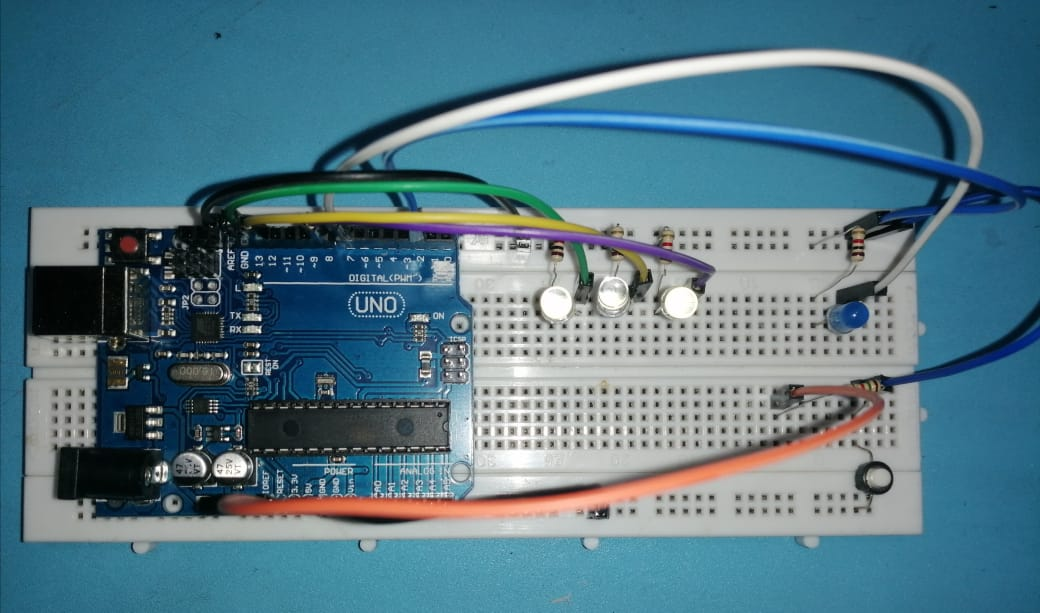
\includegraphics[width=8cm]{./imagenes/Ejemplo_01.jpeg}
\end{figure}
\newline
Donde la petición de interrupción se hace al presionar un \textit{switch} que envía una señal por medio de una caida de tensión en el pin 2 de la placa. Cuando la petición en aceptada, entonces se ``paraliza" la secuencia de parpadeo de la serie de LEDs blancos y se pone en HIGH el estado del bombillo azul. Si el \textit{switch} se vuelve a presionar, se pone en LOW el estado del LED azul y se reanuda la secuencia de los LEDs blancos.

%%%%%%%%%%%%%%%%%%%%%%%%%%%%%%%%%...................................%%%%%%%%%%%%%%%%%%%%%%%%%%%%%%%%%

\section{CONCLUSIONES}
Retomando el tema central del trabajo, el cual es exponer las interrupciones a nivel del microprocesador. Se puede concluir que las interrupciones son un mecanismo muy potente que puede acaparar amplios campos de aplicación como por ejemplo al momento de prevenir alguna catástrofe mediante algún dispositivo que detecte humo de incendio en un edificio pero que al mismo tiempo vaya haciendo otro proceso. Aunque, hay que tener en cuenta que las interrupciones en todos los microprocesadores no se realizan con la misma eficiencia e incluso en ocasiones puede haber errores ya que eso depende del lenguaje de programación y del microprocesador como tal.
\newline

%%%%%%%%%%%%%%%%%%%%%%%%%%%%%%%%%...................................%%%%%%%%%%%%%%%%%%%%%%%%%%%%%%%%%

\begin{thebibliography}{99}
\bibitem{c1} E. Santamaría, Microprocesador 68000: Hardware y software (Vol. 5), Universidad Pontificia de Comillas, 1994.
\bibitem{c2} E. Ramírez, Introducción a los microprocesadores: equipo y sistemas, Limusa, 1986.
\bibitem{c3} N. Goilav y G. Loi, Arduino: Aprender a desarrollar para crear objetos inteligentes, Barcelona: ENI, 2016.
\bibitem{c4} M. Smotherman, «Interrupts,» Julio 2017. [En línea]. Available: https://people.cs.clemson.edu/~mark/interrupts.html.
\bibitem{c5} L. Llamas, «QUÉ SON Y CÓMO USAR INTERRUPCIONES EN ARDUINO,» 28 Abril 2016. [En línea]. Available: https://www.luisllamas.es/que-son-y-como-usar-interrupciones-en-arduino/.
\bibitem{c6} M. Morris Mano, Arquitectura de computadoras, Pearson Prentice Hall, 1994.
\bibitem{c7} E. González Milanés, «INTRODUCCION A LOS MICROPROCESADORES,» 2003.
\bibitem{c8} F. Hernández Ramírez y J. D. Prades García, El software. 
\bibitem{c9} F. Reyes Cortés y J. Cid Monjaraz, «Manejo de interrupciones,» de ARDUINO. APLICACIONES EN ROBÓTICA Y MECATRÓNICA., Alfaomega.
\bibitem{c10} «Tema 9: Interrupciones,» de Estructura de computadores.
\end{thebibliography}


\end{document}